\documentclass[11pt,twoside]{article}


%\usepackage{fixltx2e} % LaTeX patches, \textsubscript
\usepackage{cmap}    % fix search and cut-and-paste in Acrobat
\usepackage{ifthen}
\usepackage[T1]{fontenc}
\usepackage[utf8]{inputenc}
%\usepackage{amsmath}
\usepackage{amsmath, amsthm, amssymb, amsbsy}
\usepackage{newtxtext,newtxmath}
%%% Custom LaTeX preamble
% PDF Standard Fonts
\usepackage{helvet}
\usepackage{courier}
\usepackage{graphicx}
\usepackage{textcomp}
\usepackage{natbib}
\usepackage{mathtools}
\usepackage{hyperref}
\usepackage{etoolbox}
\usepackage[affil-it]{authblk}

\renewcommand{\bibname}{References}
\apptocmd{\thebibliography}{\csname phantomsection\endcsname\addcontentsline{toc}{chapter}{\bibname}}{}{}



%\usepackage{fullpage} deprecated
\usepackage[left=1.25in,right=1.2in,vmargin=1.2in,headheight=110pt]{geometry}

\usepackage{verbatim}
\usepackage{enumitem}
%\setlist{nolistsep}

% header setup
\usepackage{fancyhdr}
\pagestyle{fancy}
\fancyhf{}
\fancyhead[LO]{Bay-Delta SELFE v1}
\fancyhead[LE]{Bay-Delta SELFE v1}
\fancyhead[RO]{\leftmark}
\fancyhead[RE]{\rightmark}
\fancyfoot[CE,CO]{\thepage}
\renewcommand{\headrulewidth}{0.4pt}

\hypersetup{
    colorlinks,
    citecolor=black,
    filecolor=black,
    linkcolor=black,
    urlcolor=black
}

\usepackage[acronym,toc,nomain]{glossaries}
\newglossary[slg]{symbols}{sym}{sbl}{List of Symbols}
\makeglossaries

\newacronym{selfe}{SELFE}{Semi-implicit, Eulerian-Lagrangian Finite Element Model}
\newacronym{cmop}{CMOP}{Center for Marginal Ocean Prediction}
\newacronym{vims}{VIMS}{Virginia Institute of Marine Science}
\newacronym{vof}{VoF}{Volume of Fluid}
\newacronym{fem}{FEM}{Finite Element Method}
\newacronym{elm}{ELM}{Eulerian-Lagrangian Method}
\newacronym{les}{LES}{Large Eddy Simulation}
\newacronym{gotm}{GOTM}{General Ocean Turbulence Model}
\newacronym{ctd}{CTD}{Conductivity-Temperature-Depth}
\newacronym{bdcp}{BDCP}{Bay-Delta Conservation Plan}
\newacronym{nmfs}{NMFS}{National Marine Fisheries Service}
\newacronym{cfl}{CFL}{Courant–Friedrichs–Lewy}
\newacronym{usbr}{USBR}{U.S. Bureau of Reclamation}
\newacronym{dwr}{DWR}{California Department of Water Resources}
\newacronym{d1641}{D1641}{California Water Rights Decision 1641}
\newacronym{psu}{PSU}{Practical Salinity Unit}
\newacronym{ec}{EC}{electric conductivity}
\newacronym{doc}{DOC}{Dissolved Organic Carbon}
\newacronym{ndo}{NDO}{Net Delta Outflow}
\newacronym{dsm2}{DSM2}{Delta Simulation Model 2}
\newacronym{dcc}{DCC}{Delta Cross Channel}
\newacronym{uvm}{UVM}{Ultrasonic Velocity Meter}
\newacronym{adcp}{ADCP}{Acoustic Doppler Current Profiler}
\newacronym{cwemf}{CWEMF}{California Water and Environmental Modeling Forum}
\newacronym{ebmud}{EBMUD}{East Bay Municipal Water District}
\newacronym{ccwd}{CCWD}{Contra Costa Water District}
\newacronym{swp}{SWP}{State Water Project}
\newacronym{cvp}{CVP}{Central Valley Project}
\newacronym{ccfb}{CCFB}{Clifton Court Forebay}
\newacronym{bbid}{BBID}{Byron Bethany Irrigation District}
\newacronym{dfd}{DFD}{Delta Field Division}
\newacronym{cencoos}{CenCOOS}{Central and Northern California Ocean Observing System}
\newacronym{coamps}{COAMPS}{Coupled Ocean-Atmosphere Mesoscale Prediction System}
\newacronym{narr}{NARR}{North American Regional Reanalysis}
\newacronym{tvd}{TVD}{Total Variation Diminishing}
\newacronym{detaw}{DETAW}{Delta Evapotranspiration of Applied Water}
\newglossaryentry{elev}{type=symbols,name=elev,symbol={\eta},description={Free surface elevation or stage}}


%%% User specified packages and stylesheets


%%% Macros
\newcommand{\pd}{\partial}
\newcommand{\beq}{\begin{equation}}
\newcommand{\beqa}{\begin{eqnarray}}
\newcommand{\eeq}{\end{equation}}
\newcommand{\eeqa}{\end{eqnarray}}
\newcommand{\mi}{\mbox{i}}
\newcommand{\kp}{\kappa}
\newcommand{\md}{\mbox{d}}
\newcommand{\bs}{\boldsymbol}
\newcommand{\ba}{\begin{array}}
\newcommand{\ea}{\end{array}}
\newcommand{\subphi}{\textsubscript{$\phi$}}
\providecommand{\D}{\Delta}
\providecommand{\nn}{\nonumber}
\newcommand{\sgn}{\operatorname{sgn}}
\DeclareMathOperator*{\Max}{Max}
\DeclareMathOperator*{\Min}{Min}

%%% Fallback definitions for Docutils-specific commands

\title{Hydraulic Structures in SCHISM}
\author{Eli Ateljevich}
\affil{California Department of Water Resources}
\author{Joseph Y. L. Zhang}
\affil{Virginia Institute of Marine Sciences}
\author{Kijin Nam}
\affil{California Department of Water Resources}

%%% Body
\begin{document}
\maketitle
\thispagestyle{empty}

\newcommand{\explain}[2]{\underset{\mathclap{\overset{\uparrow}{#2}}}{#1}}
\newcommand{\explainup}[2]{\overset{\mathclap{\underset{\downarrow}{#2}}}{#1}}



\tableofcontents
%\chapter{Hydraulic Structures}
%add
\section{Hydraulic structures}
\label{sec-structures}
The term {\em hydraulic structures} refers to control structures such as tidally-operated gates, 
barriers, weirs and culverts as well as to coupled boundary conditions 
representing direct transfers of water from an outflow to an inflow boundary due to mechanisms like low head pumps. 
There are numerous gates and control structures in the San Francisco Bay-Delta. Here we describe the way structures are modeled and the formulas used to calculate flow through them. 

Hydraulic structures are represented in SCHISM as paired boundary condition (Figure \ref{fig:structmesh}). Flow is calculated based on head differences at two {\em reference nodes}, one on the nominal upstream and downstream sides of the structure (but not necessarily adjoining the structure). Once the flow is calculated, it is disaggregated as a homogenous flux boundary condition over the breadth of the structure. The boundaries are enforced using a relaxation formulation, which provides some natural ramping of flow when gates that are suddenly opened or closed. Transport is coupled between the side that is an outflow and the side that is an inflow.

\begin{figure}
	\centering
		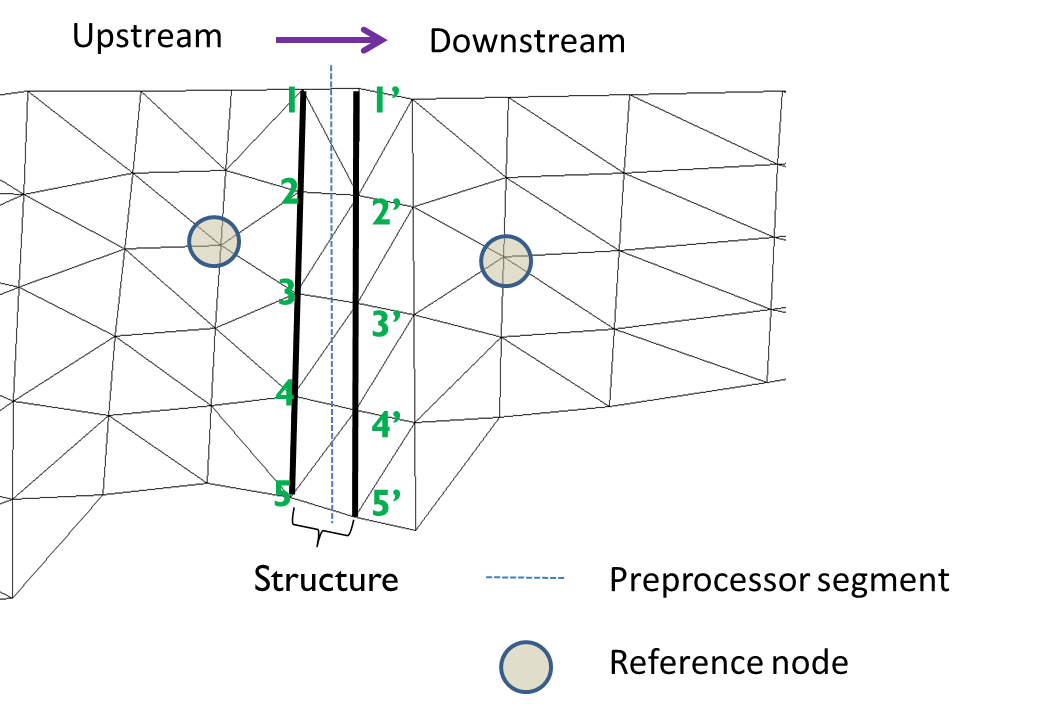
\includegraphics[scale=1]{image/struct}
	\caption{Hydraulic structure definition imposed on horizontal grid.}
	\label{fig:structmesh}
\end{figure}

A number of pre-defined flow structures are already in place covering all the cases we encountered in the Bay-Delta; with a little programming the system can easily be expanded to accommodate new structures.  
The structures we have already implemented are listed below. All of the structures admit control of key (indicated) parameters using time series. 

Structures can also be removed in SCHISM by adding 
an appropriate entry in a time series. When a structure is removed, the region between the paired boundaries reverts to the ordinary equations of motion -- ie, it is if the structure did not exist.

\subsection{Flow transfers}
\label{sec-transfer}
A flow transfer is a simple coupled boundary condition wherein a fixed flow $Q_s$ is stipulated. This flow
is imposed as an outflow boundary on one the paired boundaries and and inflow on the other. Constituent mass 
is conserved.

\begin{figure}
	\centering
		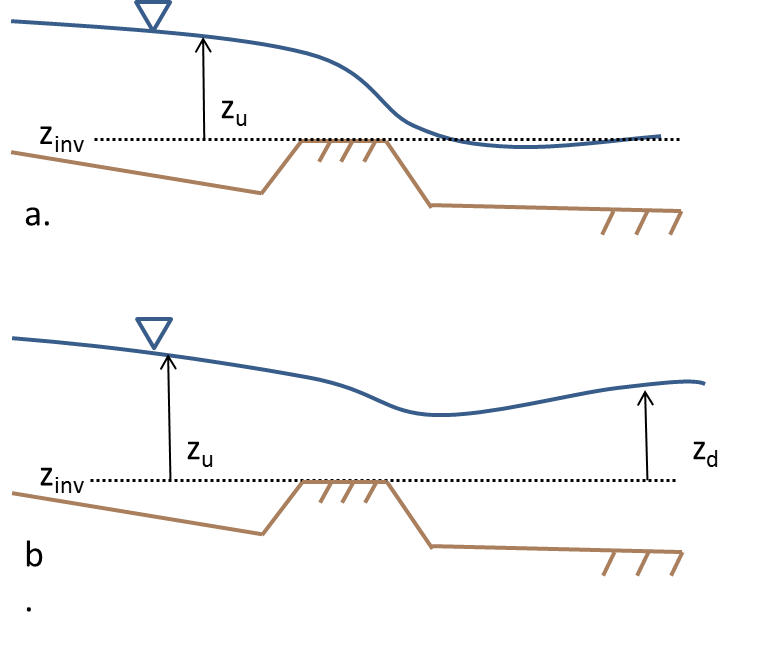
\includegraphics[scale=1]{image/weir}
	\caption{Free flowing (a) and submerged (b) weir flow cases.}
	\label{fig:weir}
\end{figure}

\subsection{Weirs}
A weir may be dry, submerged or free flowing (see Figure \ref{fig:weir}) depending on the position of the upstream
and downstream water surfaces $z_{u}$, $z_{d}$ compared to the weir invert elevation $z_{inv}$. Note that in the formulas
below, 

For the free flowing case:
$$
Q_s^f=\sgn{(z_{u} - z_{d})} C_{op} C_{f} A \sqrt{2g H}
$$
where 
\begin{align*}
&Q_s^f  &\text{free flow flow through structure (cms)} &\\
&\sgn        &\text{sign function (to induce up/downstream directionality)}  &\\
&z_u         &\text{upstream reference elevation  (m)}  &\\
&z_d         &\text{downstream reference elevation (m)}  &\\
&z_{inv}     &\text{invert elevation of the weir (m)}  &\\
&H = \max(z_u,z_d) - z_{inv}  &\text{is the energy head above the weir} &\\
&A                            &\text{area of flow (m\textsuperscript{2}) }&\\
&C_op               &\text{(directionally varying) operating coefficient (unitless)} &\\
&C_f                &\text{flow/gate coefficient (unitless)}  &\\
&g                  & \text{gravity (m/s\textsuperscript{2})} & \\
\end{align*}
For commentary on coefficients, see \cite{Rantz82}. Note that in the formulation above, the $\sqrt{2g}$
term has been kept separate and the area calculation uses water surface height. 
Furthermore, note that $z_u$ and $z_d$ are pre-assigned upstream and downstream orientations,
whereas $H$ is the energy head in the direction that is upstream of the weir in terms of actual flow.

The submerged case is derived from the free flowing case using the correction given by \citet{Villemonte47}:
\begin{align*}
Q_s^s = Q_s^f(1 - S^{1.5})^{0.385} \\
S = \frac{\min(z_u,z_d) - z_{inv}}{\max(z_u,z_d) - z_{inv}}
\end{align*}
in terms of the {\em submergence ratio} $S$.

If both sides are dry, of course $Q_s=0$ for the structure. Note that this refers to being dry with respect to the invert elevation.
The nodes may not go dry in the ordinary sense with respect to the bed -- this is the same restriction as at other SCHISM boundaries. 

\subsection{Radial gates} 
\label{sec:radial}
A radial gate is parametrized as shown in Figure \ref{fig:radial}, although at the moment we have ignored the kinetic 
energy component of upstream head (so that $H_1 = y_1$). For the case where the radial gate is completely out
of the water or the tailwater elevation is not sufficiently high to affect the upstream (submergence ratio described in the previous
section is less than $S_p=0.66$),
the gate reverts to a modified weir equation described momentarily. For the case where the radial gate is completely submerged 
(submergence ratio greater than $S_f=0.80$),
the gate is treated as an orifice as given in Section \ref{sec-orifice}.

            %diff = max_elev - min_elev
            %coef_matching_factor = sqrt(1.d0/(1.d0-PART_SUBMERGE))
            %flow = signed_coef*area*sqrt2g*sqrt(diff)
            %! now weigh the two so that the flow makes a linear transition
            %subfrac = (submerge_ratio-PART_SUBMERGE)/(FULL_SUBMERGE - PART_SUBMERGE)
            %flow = ((1.d0 - subfrac)*coef_matching_factor + subfrac)*flow
For free flow:
$$
Q_s^f = \sgn{(z_{u} - z_{d})} C_{op} C_{f} A \sqrt{2g H}
$$
and for partially submerged flow ($S_p < S \le S_f$):
$$
Q_s^p = \sgn{(z_{u} - z_{d})} C_{op} C_{f} A \sqrt{2g \left|\D z\right|}[(1-\hat{S})m+\hat{S}]
$$
where
\begin{align*}
&\hat{S}=\frac{S-S_p}{S_f-S_p} & \text{is the submergence fraction} \\
&m = \sqrt{\frac{1}{1-S_p}} & \text{is a coefficient matching factor to create a smooth transition}. \\
\end{align*}

For fully submerged flow $S>S_f$, the orifice equation is used. This is equivalent to the submerged equation with
$\hat{S}=1$.


\begin{figure}
	\centering
		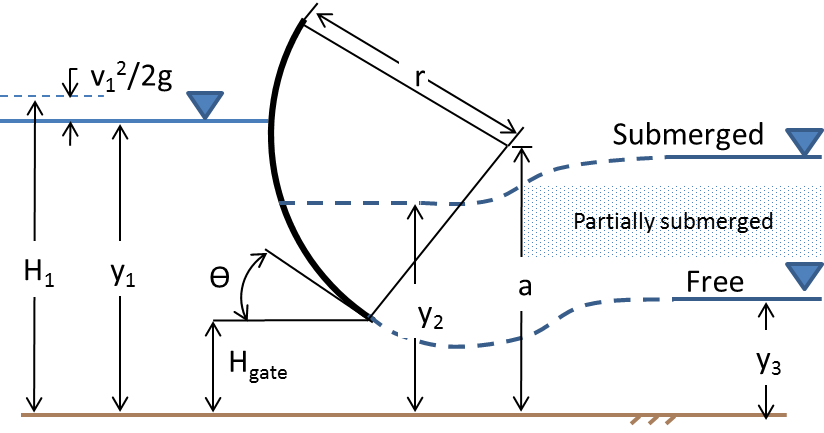
\includegraphics[scale=1]{image/radial_gate}
	\caption{Radial gate.}
	\label{fig:radial}
\end{figure}

\subsection{Radial gates with linear coefficient} 
This is an alternative radial gate formula modified from a suggestion by Tony Wahl of the USBR (personal communication) 
that was incorporated because it matches Clifton Court well. 
The rating formula is a little simpler, but the flow coefficient is a linear function of gate height:

$$
Q_s = \sgn{(z_{u} - z_{d})} C_{op} C_{f} A \sqrt{2g \left|\D z\right|}
$$
where
$$C_f = d + sR$$
is the gate coefficient linearly dependent on the ratio of gate opening to upstream head:
$$R = \min(\frac{H_{gate}}{H_1},1.0)$$
with constant and linear parameters $d$ and $s$ respectively.
Some special cases surround the term $A$, given that the top of the radial gate
may be dry or submerged.

\subsection{Orifice}
\label{sec-orifice}
The orifice option is used to model a sluice gate or flashboard or other devices that  
presents a (rectangular) apertures to flow. Flow in this case is given by:

$$
Q_{s} = \sgn{(z_{u} - z_{d})} C_{op} C_{f} A \sqrt{2g \left|\D z \right|}
$$

Some special cases surround the term $A$, given that the orifice may be dry, partially submerged or completely
submerged. Typically, the orifice equation is most useful when flow is fully submerged.

\subsection{Culverts}
A culvert is currently modeled as a circular orifice. In other words, it is the same as the orifice case
but with a different formula for $A$. This treatment neglects some of the nuances of head and tailwater control 
as described by \cite{Bodhaine68}




\section{Model Input for Structures}
\subsection{Enabling Structures ({\em param.in})}
Hydraulic stuctures are enabled in \url{param.in} using the parameter {\em ihydraulics}. This is a binary
flag with 1 indicating that structures are to be used and 0 indicating that they will be ignored.

\subsection{Defining Structures ({\em hydraulics.in})}
Below is an annotated example \url{hydraulics.in} file. The line numbers are not part of the original file
and the comments (parts after the "`!"') are not required.

\begin{samepage}
\verbatiminput{hydraulics.in}
\end{samepage}
\subsubsection{Global header (example line 1-2)}
The first two lines of \url{hydraulics.in} include two global parameters, 
the total number of structures and the nudging factor.

The gate equations are not enforced exactly. We have found that this specification is not fully stable, particularly when gates
are abruptly installed or open. Instead we use a relaxation formulation:

$$Q(t+\frac{\Delta t}{2})= (1-\chi) Q(t) + (\chi) Q_{\text{s}}(\eta(t),\mathbf{u}(t),\phi(t+1))$$

where $Q_s$ is the explicit flow calculation for the structure based on state variables and parameters at time $t$.

In other words, rather than being set exactly to the gate value, the (coupled) flow boundaries will be nudged a fraction $\chi$ towards this value. 
The nudging factor can also be interpreted as a time constant. Using a small value like 0.1 will provide maximum stability, but is too slow
to respond to tidal fluctuations. 

\subsubsection{Structure geometry}
After the global parameters, the next lines (3-10 in the example) represent the identification and geometry of the structure:
\begin{enumerate}
\item [Line 3] An index and name for the structure. The indices must be sequential and the maximum length of name is 32 characters
\item [Line 4] The number of node pairs in the definition, the upstream reference node and the downstream reference node. All use global node numbers.
\item [Line 5-10] For each node pair in the string defining the structure, the member of the pair on the upstream and downstream side. 
The start and end must be on land boundaries. The concept of a node pair is illustrated by the unprimed and primed nodes in Figure \ref{fig:structmesh}
\end{enumerate}

\subsubsection{Parameters and coefficients}
\label{sec:gate_spec}
After the geometric information are some parameters that are specific to the structure type.
In the example, this happens to fall on lines 11-14 although this would be different with different geometry
or in a \url{hydraulics.in} with multiple gates.
The first of these lines controls this input with the structure type being listed on the first of these lines. 
All parameters are specified {\em per unit}. For all structures except the hydraulic tranfer, 
the number of duplicate units is controlled by the variable {\em nduplicate}. 

Many of the structures have invert elevations among their parameters. The datum for this elevation is the same
as the datum for the elevation state variable $\eta$ in the model.

\paragraph{transfer}
A transfer is a coupled boundary condition (outflow and inflow). The only parameter is the prescribed flow.
\begin{verbatim}
struct_type        ! type of structure (transfer)
nduplicate         ! number of duplicate units
flow               ! flow in cms
\end{verbatim}

\paragraph{orifice,radial}
\begin{verbatim}
struct_type        ! type of structure (orifice, radial)
nduplicate         ! number of duplicate units
elev width height  ! invert elevation (m), width, height (rectangular)
coef op_down op_up ! flow coeficient, operating coefficient down and up
\end{verbatim}

\paragraph{radial\_rh}
A {\em radial\_rh} gate has a flow coefficient that has both
a constant term and a linear variation in the gate height:
\begin{verbatim}
struct_type        ! type of structure (radial_rh)
nduplicate         ! number of duplicate units
elev width height  ! invert elevation (m), width (m), height (m)
coef coef_linear   ! constant, linear height-based parameters of flow coef.
op_down op_up      ! op coef down/up
\end{verbatim}

\paragraph{weir}
An orifice is submerged, rectangular orifice (outflow and inflow). 
\begin{verbatim}
struct_type        ! type of structure (weir)
nduplicate         ! number of duplicate units
elev width height  ! invert elevation, width of  a single unit, height
coef op_down op_up ! flow coef., operating coefficients down and up
\end{verbatim}

\paragraph{culvert}
An culvert is a round culvert
\begin{verbatim}
struct_type        ! type of structure (culvert)
nduplicate         ! number of duplicate units
elev width         ! invert elevation, radius
coef op_down op_up ! flow coeficient, operating coeficient down and up
\end{verbatim}

\paragraph{weir\_culvert}
This is a combination of weir and culvert
\begin{verbatim}
struct_type           ! type of structure (culvert)
weir_nduplicate       ! number of duplicate weir units
weir_elev weir_width  ! invert elevation, radius
weir_coef weir_op_down weir_op_up ! flow, operating coefs for weir
pipe_nduplicate       ! number of duplicate culvert/pipe units
pipe_elev pipe_width              ! invert elevation, radius
pipe_coef pipe_op_down pipe_op_up ! flow, operating coefs for culvert
\end{verbatim}

\subsubsection{Enabling time series control}
\label{sec:timeflag}
The final line (line 15 in the example) of each structure definition is a flag (1=True, 0=False) indicating whether a time history (\url{*.th}) file will be used to make many of the parameters time-varying -- effectively replacing the values loaded in 
\url{hydraulics.in}. Time series control is covered in Section \ref{sec:timeseries}.

\subsection{Time Series Files ({\em *.th})}
\label{sec:timeseries}
If you set the time series flag for a gate coefficient to 1=True as indicated in \ref{sec:timeflag}, time series control is
enabled for the gate. You need to provide an input file named \url{[gate_name].th} where {\em [gate\_name]} 
is identical to the name used in the gate definition.

The file \url{[gate_name].th} is a multivariate time history.As with all \url{*.th} files the first column  is time in elapsed seconds since the start of the run and the other columns are space delimited.
One quirk compared to other SCHISM inputs is that the times can be irregular and interpolation 
for gate variables is based on constant repetition of the previous value, not on linear interpolation. This, we feel, is more typical of the actuator on a gate; some things (like "`installation"') are
also not meaningful at intermediate values.

The other parameters that are included depend on the gate type, and the columns for each type are given below. 
Most of the variables are identical to the ones listed in \url{hydraulics.in} and described in
Section \ref{sec:gate_spec}. Howerver, there is one special variable {\em install} that is always 
located in the column immediately after the time column. This variable takes on integer values and must be zero or one. 
Setting the installation to zero removes the structure, restoring the original algorithm.
 
\begin{description}
\item[transfer] time  install(int) flow    ! Install = \(0,1\)
\item[culvert,weir] time install(int) nduplicate(int) op\_down op\_up elev width
\item[orifice,radial,radial\_rh] time install(int) nduplicate(int) op\_down op\_up elev width height
\item[weir\_culvert] time install (int) ndup\_weir (int) op\_down\_weir op\_up\_weir elev\_weir width\_weir ndup\_pipe (int) down\_op\_pipe up\_op\_pipe elev\_pipe radius\_pipe
\end{description}

Below is a sample \url{dcc.th}, corresponding to the radial gate used in the original example \url{hydraulics.in}:
\begin{samepage}
\verbatiminput{dcc.th}
\end{samepage}




\bibliography{references}
 \bibliographystyle{plainnat}
\printglossaries
\end{document}
